\documentclass[tikz,border=2pt]{standalone}

\usepackage{pgfplots}
\pgfplotsset{compat=1.18}

\begin{document}
	
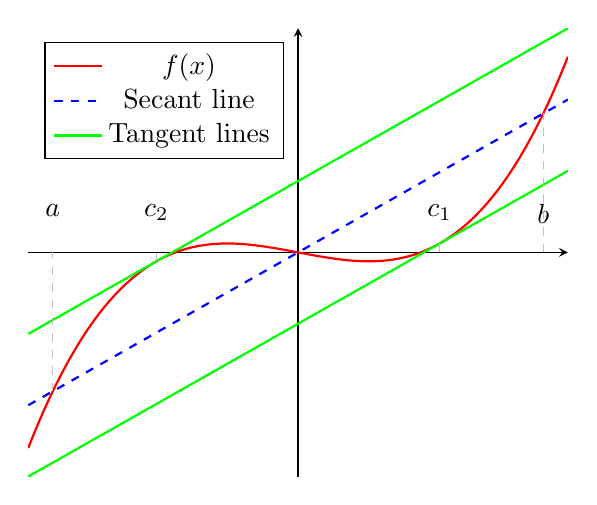
\begin{tikzpicture}
	\begin{axis}[
		axis lines = middle,
		legend pos = north west,
		xtick=\empty, 
		ytick=\empty,
		legend style={at={(0.03,0.97)},anchor=north west},
		]
		
		% Define the function
		\addplot[
		domain=-2.2:2.2, 
		samples=100, 
		color=red,
		thick,
		]
		{x^3 - x};
		\addlegendentry{\(f(x)\)}
		
		% Define points a, b, and c1, c2
		\def\pointA{-2}
		\def\pointB{2}
		\def\pointCone{1.1547}
		\def\pointCtwo{-1.1547}
		
		% Add nodes for a, b, and c1, c2
		\node[coordinate,label=below:\(a\)] at (axis cs:\pointA,2.5) {};
		\node[coordinate,label=below:\(b\)] at (axis cs:\pointB,2.5) {};
		\node[coordinate,label=below:\(c_1\)] at (axis cs:\pointCone,2.5) {};
		\node[coordinate,label=below:\(c_2\)] at (axis cs:\pointCtwo,2.5) {};
		
		% Draw secant line
		\addplot[dashed, color=blue, thick, domain=-2.2:2.2] {(\pointB^3 - \pointA^3 - \pointB + \pointA)/(\pointB - \pointA)*x + \pointA^3 - \pointA - (\pointB^3 - \pointA^3 - \pointB + \pointA)/(\pointB - \pointA)*\pointA};
		\addlegendentry{Secant line}
		
		% Draw tangent lines at c1 and c2
		\addplot[domain=-2.2:2.2, thick, color=green] {3*x - 3.08};
		\addplot[domain=-2.2:2.2, thick, color=green] {3*x + 3.08};
		\addlegendentry{Tangent lines}
		
		% Draw dashed lines for a, b, and c1, c2
		\addplot[dashed,color=lightgray] coordinates {(\pointA, -6) (\pointA, 0)};
		\addplot[dashed,color=lightgray] coordinates {(\pointB, 0) (\pointB, 6)};
		\addplot[dashed,color=lightgray] coordinates {(\pointCone, 0.38489856432) (\pointCone, 0)};
		\addplot[dashed,color=lightgray] coordinates {(\pointCtwo, -0.38489856432) (\pointCtwo, 0)};
	\end{axis}
\end{tikzpicture}
	
\end{document}